\message{ !name(lab.tex)}\documentclass[a4paper,12pt]{article}

\usepackage[T2A]{fontenc}
\usepackage[utf8]{inputenc}
\usepackage[russian]{babel}
\usepackage{cmap}

\usepackage{xcolor}

\usepackage{helvet}
\usepackage{pscyr}


\usepackage{multicol}

% \usepackage{amssymb,amsfonts,amsmath,mathtext}
% \usepackage{cite,enumerate,float}

\graphicspath{{images/}}		% Подключаемые пакеты
%%% Макет страницы %%%
\geometry{a4paper,top=20mm,bottom=27mm,left=30mm,right=15mm}
\setstretch{1.15}

%%% Язык текста %%%
\selectlanguage{russian}

%%% Кодировки и шрифты %%%
\renewcommand{\rmdefault}{ftm} % Включаем Times New Roman

%%% Выравнивание и переносы %%%
\sloppy				% Избавляемся от переполнений
\clubpenalty=10000		% Запрещаем разрыв страницы после первой строки абзаца
\widowpenalty=10000		% Запрещаем разрыв страницы после последней строки абзаца
\interfootnotelinepenalty=10000 % Запрет разрывов сносок

%%% Нумерация страниц %%%
\fancypagestyle{empty}{%
\fancyhf{} % clear all header and footer fields
\renewcommand{\headrulewidth}{0pt}
\renewcommand{\footrulewidth}{0pt}
\setlength{\headheight}{5mm} 
}

\fancypagestyle{plain}{%
\fancyhf{} % clear all header and footer fields
\fancyfoot[R]{\thepage} 
\renewcommand{\headrulewidth}{0pt}
\renewcommand{\footrulewidth}{0pt}
\setlength{\headheight}{5mm}
}

\pagestyle{plain}

%%% Библиография %%%

\makeatletter
\bibliographystyle{ugost2003s} % Оформляем библиографию в соответствии с ГОСТ 7.1 2003

\let\oldthebibliography=\thebibliography
\let\endoldthebibliography=\endthebibliography
\renewenvironment{thebibliography}[1]{
  \begin{oldthebibliography}{#1}
    \setlength{\parskip}{0mm}
    \setlength{\itemsep}{0mm}
}
{
\end{oldthebibliography}
}

%%% Изображения %%%
\graphicspath{{images/}} % Пути к изображениям

%%% Содержание %%%
\renewcommand{\cfttoctitlefont}{\hfil \large\bfseries}

\setlength{\cftparskip}{0mm}
\setlength{\cftbeforesecskip}{0mm}
\setlength{\cftaftertoctitleskip}{14pt}

\renewcommand{\cftsecaftersnumb}{\:}
\renewcommand{\cftsecfont}{}   
\renewcommand{\cftsecpagefont}{\normalsize}
\renewcommand{\cftsecleader}{\cftdotfill{\cftdotsep}}
\setlength{\cftsecindent}{0mm}
\setlength{\cftsecnumwidth}{3mm}

\setlength{\cftsubsecindent}{4mm}
\setlength{\cftsubsecnumwidth}{8mm}

%%% Требования ЕСКД/СТП %%%

%%% Размеры заголовков
\newcommand{\sectionbreak}{\clearpage}

\titleformat{\section}{\large\bfseries}{\thesection}{\wordsep}{}
\titlespacing*{\section}{12mm}{14pt}{14pt}

\titleformat{name=\section,numberless}{\large\bfseries\filcenter}{}{0mm}{}
\titlespacing*{name=\section,numberless}{0mm}{14pt}{14pt}

\titleformat{name=\subsection}{\normalsize\bfseries}{\thesubsection}{\wordsep}{}
\titlespacing*{\subsection}{12mm}{14pt}{14pt}

\titleformat{name=\subsection,numberless}{\normalsize\bfseries}{}{0mm}{}
\titlespacing*{name=\subsection,numberless}{0mm}{14pt}{14pt}

%%% Нумерация параграфов

\counterwithout{paragraph}{subsubsection}
\counterwithin{paragraph}{subsection}
\renewcommand{\theparagraph}{\thesubsection.\arabic{paragraph}}
\setcounter{secnumdepth}{4}

\titleformat{name=\paragraph}[runin]{\normalsize\bfseries}{\theparagraph}{\wordsep}{}
\titlespacing*{\paragraph}{12mm}{14pt}{\wordsep}

%%% Размеры текста формул %%%

\DeclareMathSizes{12}{12}{6}{4}

%%% Расстояние между формулами

\AtBeginDocument{%
  \setlength\abovedisplayskip{14pt}%
  \setlength\belowdisplayskip{14pt}%
  \setlength\abovedisplayshortskip{14pt}%
  \setlength\belowdisplayshortskip{14pt}%
}

%%% Оформление текста

\setlength{\parskip}{0pt}
\setlength{\parindent}{12mm}

%%% Расстояние между плавающими элементами

\setlength{\floatsep}{14pt}     % between top floats
\setlength{\textfloatsep}{14pt} % between top/bottom floats and text
\setlength{\intextsep}{14pt}    % between text and float
\setlength{\dbltextfloatsep}{14pt}
\setlength{\dblfloatsep}{14pt}

 % костыль для того, чтобы убрать расстояние от картинки до текста
\setlength{\abovecaptionskip}{0pt}
\setlength{\belowcaptionskip}{0pt}
           
%%% Оформление списков
\AddEnumerateCounter{\asbuk}{\@asbuk}{\cyrm}

\setlist{nosep,listparindent=\parindent}
\setlist[1]{itemindent=18.5mm,leftmargin=0mm,itemsep=0mm,topsep=0mm,parsep=0mm}             
\setlist[itemize,1]{label=$-$}
\setlist[enumerate,1]{label=\arabic*)}

\setlist[2]{itemindent=20.5mm,leftmargin=0mm,itemsep=0mm,topsep=0mm,parsep=0mm}             

% Определяем новый стиль для списков,
% на которые есть ссылки в тексте
\newlist{reflist}{enumerate*}{1}
\setlist*[reflist,1]{%
  label=\asbuk*),
}

\setlist*[reflist,2]{%
  label=\arabic*),
}

%% Нумерация плавающих элементов

\counterwithin{figure}{section}
\counterwithin{table}{section}

\makeatletter
\AtBeginDocument{%
\renewcommand{\thetable}{\thesection.\arabic{table}}
\renewcommand{\thelstlisting}{\thesection.\arabic{lstlisting}}
\renewcommand{\thefigure}{\thesection.\arabic{figure}}
\let\c@lstlisting\c@figure}
\makeatother 

%% Подписи плавающих элементов

\captionsetup[figure]{
  labelsep=endash,
  justification=centering,
  singlelinecheck=false,
  position=bottom,
  skip=14pt}

\captionsetup[table]{
  labelsep=endash,
  justification=raggedright,
  singlelinecheck=false,
  position=top,
  skip=0mm}

\captionsetup[lstlisting]{
  labelsep=endash
}

\lstset{
basicstyle=\scriptsize\ttfamily,
numberstyle=\scriptsize\ttfamily,
keywordstyle=\bfseries,
commentstyle=\itshape,
numbers=left,
stepnumber=1,
frame=single,
resetmargins=true,
xleftmargin=7mm,
xrightmargin=2mm,
captionpos=b,
keepspaces=true,
breaklines=true,
aboveskip=22pt,
belowskip=10pt,
abovecaptionskip=16pt}

\renewcommand{\arraystretch}{1.5}

%%% Настройка размеров вертикальных отступов

\renewcommand{\smallskip}{\vspace{6pt}}
\renewcommand{\bigskip}{\vspace{14pt}}
			% Пользовательские стили

\begin{document}

\message{ !name(lab.tex) !offset(-3) }


%%% Переопределение именований %%%
\renewcommand{\abstractname}{Аннотация}
\renewcommand{\alsoname}{см. также}
\renewcommand{\appendixname}{Приложение}
\renewcommand{\bibname}{Литература}
\renewcommand{\ccname}{исх.}
\renewcommand{\chaptername}{Глава}
\renewcommand{\contentsname}{СОДЕРЖАНИЕ}
\renewcommand{\enclname}{вкл.}
\renewcommand{\figurename}{Рисунок}
\renewcommand{\lstlistingname}{Рисунок}
\renewcommand{\headtoname}{вх.}
\renewcommand{\indexname}{Предметный указатель}
\renewcommand{\listfigurename}{Список рисунков}
\renewcommand{\listtablename}{Список таблиц}
\renewcommand{\pagename}{Стр.}
\renewcommand{\partname}{Часть}
\renewcommand{\seename}{см.}
\renewcommand{\tablename}{Таблица}

\renewcommand{\refname}{СПИСОК ИСПОЛЬЗОВАННЫХ ИСТОЧНИКОВ}
			% Переопределение именований

\thispagestyle{empty}
\setlength{\parindent}{0ex} % set paragraph indenting to zero

\begin{center}
  Министерство образования Республики Беларусь \\
  \vspace{0.5ex}
  Учреждение образования \\
  БЕЛОРУССКИЙ ГОСУДАРСТВЕННЫЙ УНИВЕРСИТЕТ \\
  ИНФОРМАТИКИ И РАДИОЭЛЕКТРОНИКИ \\
  \vspace{0.5ex}
  Факультет информационных технологий и управления \\
  \vspace{0.5ex}
  Кафедра информационных технологий автоматизированных систем
\end{center}

\vspace{50mm}

\begin{center}
  Отчет по лабораторной работе № 4 \\
  <<Модульное программирование на языке Ассемблер>>
\end{center}

\vspace{60mm}

\begin{minipage}{.55\linewidth}
    Выполнил студент группы 120602

    \smallskip

    Проверил
\end{minipage}
\hfill
\begin{minipage}{.4\linewidth}
  \begin{flushright}
    Будный Р. И. \_\_\_\_\_\_\_\_\_\_

    \smallskip

    Гончаревич А. Л. \_\_\_\_\_\_\_\_\_\_
  \end{flushright}
\end{minipage}

\vspace{50mm}
\begin{center}
  Минск 2014
\end{center}

\setlength{\parindent}{1.25cm} % reset paragraph indenting

\newpage
			% Титульный лист

\section{ЦЕЛЬ РАБОТЫ}

Цели данной лабораторной работы:

\begin{itemize}
\item
  ознакомление с параметрической формой задания случайных процессов;
\item
  приобретение навыков расчета математических ожиданий, дисперсий, 
  ковариационных и взаимных ковариационных функций случайных процессов.
\end{itemize}
            % Цели работы
\section{Исходные данные}
\addcontentsline{toc}{section}{Исходные данные}	% Добавляем его в оглавление

\begin{figure}[h!t]
  		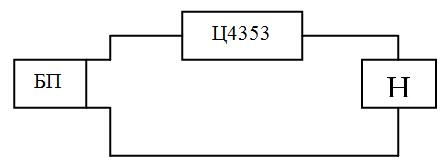
\includegraphics[width=0.4\linewidth]{scheme1}
  		\centering{\caption{Схема усилительного каскада}}
\end{figure}

     % Приборы, используемые в работе
\section{Теоретические сведения}
\addcontentsline{toc}{section}{Теоретические сведения}	% Добавляем его в оглавление

Инструментальная погрешность имеет различные формы: абсолютную ($ \Delta $), относительную ($ \delta $) и приведённую ($ \gamma $):

\begin{equation*}
  \label{eq:equation1}
  \Delta_{i} = \vert X_{i} - Q \vert
\end{equation*}

\begin{equation*}
  \label{eq:equation2}
  \delta_{i} = \dfrac{\Delta_{i}}{Q} * 100\% = \gamma_{i} * \dfrac{X_{N}}{Q}
\end{equation*}

\begin{equation*}
  \label{eq:equation3}
  \gamma_{i} = \dfrac{\Delta_{i}}{X_{N}}*100\%
\end{equation*}

\noindent где $ X_{N} $ -- нормируемое значение, которое согласно ГОСТ 8.401-80 следует выбирать равным пределу измерения,

$ Q $ -- действительное значение величины,

$ X_{i} $ -- показание прибора.

\vspace{4mm}

Входное сопротивление $ R_{V} $ и входная емкость $ C_{V} $ вольтметра B7-28 определяется по следующим формулам:

\begin{equation*}
  \label{eq:equation4}
  R_{V} = R_{0} * \dfrac{U_{R_{V}} - 1}{U_{G_{H}}}
\end{equation*}

\begin{equation*}
  \label{eq:equation5}
  C_{V} = C_{0} * ( \dfrac{U_{G_{B}}}{U_{C_{V}}} - 1)
\end{equation*}

\noindent где $ R_{V} $ -- активное сопротивление,\par
$ C_{V} $ -- входная емкость,\par
$ U_{C_{V}} $, $ U_{R_{V}} $ -- показания вольтметра,\par
$ U_{G_{H}} $ -- напряжение генератора на нижней частоте,\par
$ U_{G_{B}} $ -- напряжение генератора на верхней частоте,\par
$ C_{0} $, $ R_{0} $ -- известные сопротивление и емкость, включенные в схему.\par

\vspace{4mm}

Коэффициенты амплитуды $ K_{a} $ и формы $ K_{f} $ рассчитываются по формулам:

\begin{equation*}
  \label{eq:equation6}
  K_{f} = \dfrac{U_{CK}}{U_{CB}}
\end{equation*}

\begin{equation*}
  \label{eq:equation4}
  R_{a} = \dfrac{U_{m}}{U_{CK}}
\end{equation*}

\begin{figure}[h]
  \center{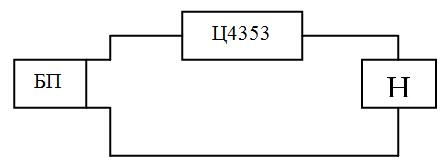
\includegraphics[width=0.8\linewidth]{scheme1}}
  \caption{Принципиальная схема установки}
\end{figure}


\vspace{4mm}

\begin{table} [htbp]
  \begin{center}
    \begin{tabular}{ p{5cm} p{5cm} p{5cm}l }

      \centering B4-12 \par &\centering B3-40 &\centering B3-38 & \\
      \centering $ U_{m} = U_{V} $ \par &\centering $ U_{CK} = U_{V} $ &\centering $ U_{CB} = U_{V}/1.11 $ & \\
      \centering $ \delta_{B4-12} = \gamma * \dfrac{U_{pr. B4-12}}{U_{B4-12}} $ \par
      &\centering $ \delta_{B3-40} = \gamma * \dfrac{U_{pr. B3-40}}{U_{B3-40}} $ 
      &\centering $ \delta_{B3-38} = \gamma * \dfrac{U_{pr. B3-38}}{U_{B3-38}}$ & \\

      \centering $ \gamma = \pm 4 \% $ &\centering $ \gamma = \pm 1,5 \% $ \par &\centering $ \gamma = \pm 2,5 \% $ \\ 

    \end{tabular}
  \end{center}
\end{table}



\clearpage
	    % Теоретические сведения   
\section{ХОД РАБОТЫ}

\subsection{Формулировка задачи}

Рассчитать функции математического ожидания, дисперсии и ковариационной функции
случайного процесса $ \zeta(t) $. Вид составляющих случайного процесса
и распределения их параметров:
$ \zeta(t)= \xi(t) + \psi(t) $,
$ \xi(t) = b $,
$ b \in N(a_b, \sigma^2_b) $,
$ \psi(t) = A \cdot cos(\omega_1 t + \varphi) $,
$ \varphi \in U(-a,a)$.

В символьных расчетах параметры $ b, c, d,
\varphi, \omega_1 $ рассматривать как символьные переменные.

В одно графическое окно вывести десять реализаций случайного процесса $ \zeta(t) $
и функции математического ожидания и дисперсии, выбрав значения
параметров $ b, c, d, \varphi, \omega_1 $.

В отдельное графическое окно вывести график ковариационной функции
случайного процесса $ \zeta(t) $ при выбранных значениях неслучайных параметров.


\subsection{Теоретические сведения}

Математическое ожидание $ a_{\zeta} (t) $, дисперсия $ d_{\zeta} (t) $,
ковариационная функция $ R_{\zeta} (t_1, t_2) $ случайного процесса $ \zeta(t) $
при условии, что $ \zeta(t) = \xi(t) + \psi(t) $ и случайные процессы $ \xi(t) $
и $ \psi(t) $ определены своими конечномерными плотностями вероятностей, рассчитываются
следующим образом:
\begin{align*}
  a_{\xi}(t) &= \int\limits_{-\infty}^{+\infty}  \xi(t, z) f_{\lambda}(z) dz, \\ 
  D_{\xi}(t) &= \int\limits_{-\infty}^{+\infty} (\xi(t, z) - a_{\xi}(t))^2 f_{\lambda}(z) dz, \\
  R_{\xi}(t_1, t_2) &= \int\limits_{-\infty}^{+\infty} \int\limits_{-\infty}^{+\infty} (\xi(t_1, z) - a_{\xi}(t_1)) (\xi(t_2, z) - a_{\xi}(t_2)) f_{\lambda}(z) dz. \\
\end{align*}


\pagebreak
\subsection{Ход работы}

Для выполнения лабораторной работы воспользуемся языком программирования
\textit{Python} и несколькими библиотеками этого языка:
для выполнения символьных вычислений математического ожидания, дисперсии и
ковариационной функции случайного процесса $ \zeta(t) $ воспользуемся библиотекой
\textit{sympy}, для подстановки численных значений вместо параметров и отображения функций
на графиках будем использывать библиотеки \textit{numpy} и \textit{matplotlib} соответственно.

Исходный код разработанной программы представлен в приложении~А.


В одно графическое окно выведем десять реализаций случайного процесса $ \zeta(t) $,
его функции математического ожидания и дисперсии. В качестве параметров будем использывать
следующие величины: $ A = 2 $, $ w_1 = 1 $, $ \varphi \in (-\frac{\pi}{2}; \frac{\pi}{2}) $,
$ t \in (0, 10) $ с шагом $ 0{,}2 $ с. Полученные графики приведены на рисунке~\ref{pic:values}.
\begin{figure}[h]
  \centering
  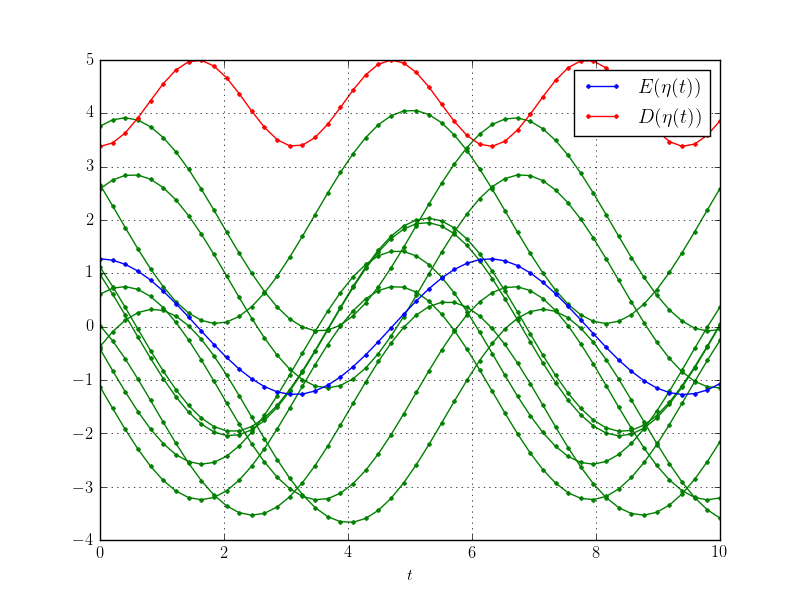
\includegraphics[width=150mm, height=92mm]{pic/values}
  \caption{Графики десяти реализаций, математического ожидания и дисперсии случайного процесса $ \zeta(t) $}
  \label{pic:values} 
\end{figure}

\pagebreak

График ковариационной функции случайного процесса $ \zeta(t) $ приведен на рисунке~\ref{pic:correlation}.
\begin{figure}[h]
  \centering
  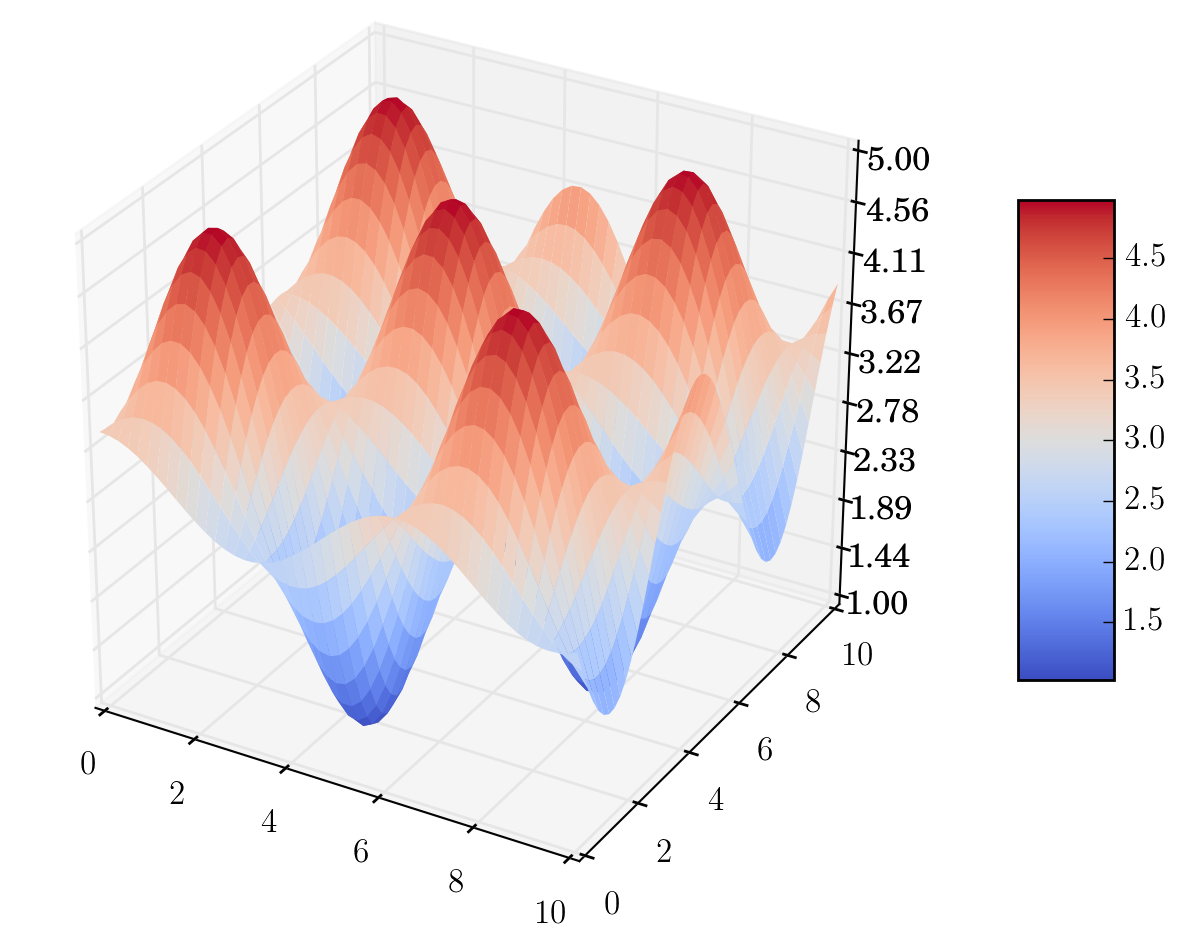
\includegraphics[width=150mm, height=92mm]{pic/correlation}
  \caption{График ковариационной функции \\ случайного процесса $ \zeta(t) $}
  \label{pic:correlation} 
\end{figure}
 
\newpage
         % Ход работы


\addcontentsline{toc}{section}{Заключение}
\section*{ЗАКЛЮЧЕНИЕ}

В ходе дипломного проекта было выполнено проектирование и программная реализация
модуля для отображения актуальной финансовой информации на мобильных устройствах
под управлением операционной системы iOS. Был произведен сравнительный
анализ источников финансовой информации, в ходе которого был найден
веб-ресурс, предоставляющий необходимую информацию для приложения на
бесплатной основе.

Разработанный программный продукт предоставляет пользователю информацию о курсах
валют в Республике Беларусь в зависимости от выбранного областного центра,
возможность формирования списка избранных отделений.
Предусмотрена работа мобильного приложения без подключения к сети Интернет.

Пользователю доступен экран конвертера валют, предоставляющий возможность
конвертации валюты с использованием как курса Национального банка Республики
Беларусь, так и курсов, установленных в коммерческих банках нашей страны.

В целях наглядного отображения, финансовая информация разбивается
по категориям, проходит этапы фильтрации и сортировки. В качестве дополнительной
информации, рассчитываются значения среднего, наилучшего курса обмена валют,
а также количество отделений коммерческих банков, предоставляющих информацию о
выбранном курсе.

С целью дальнейшего совершенствования разработанного программного модуля,
была рассмотрена перспектива и необходимость разработки новых версий,
намечены направления развития приложения.

Разработанный программный модуль доступен для скачивания в магазине приложений
App Store на бесплатной основе.
		% Заключение

\end{document}



\message{ !name(lab.tex) !offset(-27) }
